\documentclass{article}

\usepackage{graphicx}
\usepackage{xcolor}
\usepackage{indentfirst}
\usepackage{booktabs}
\usepackage[a4paper, total={6in, 8in}]{geometry}
\usepackage{hyperref}
\usepackage{fancyhdr}
\usepackage{subcaption}
\usepackage{xepersian}
\usepackage{fontspec}
\usepackage{url}
\settextfont[Scale=1.2,ExternalLocation=fonts/,BoldFont=B Nazanin Bold.ttf]{B Nazanin}
\setlatintextfont[Scale=1.2,ExternalLocation=fonts/,BoldFont=XB Zar.ttf]{Times New Roman}

\definecolor{codegray}{gray}{0.9}
\newcommand{\code}[1]{\colorbox{codegray}{\texttt{\lr{#1}}}}

\begin{document}


%title page%
\begin{titlepage}
	\begin{center}
		\vspace{0.2cm}
		
		
\includegraphics[width=0.4\textwidth]{sharif.png}\\
		\vspace{0.5cm}
		\textbf{ \Huge{پروژه شبیه‌سازی کامپیوتری}}\\
		\vspace{0.25cm}
		\textbf{ \Large{دکتر بردیا صفایی}}
		\vspace{0.2cm}
		
		
		\large \textbf{دانشکده مهندسی کامپیوتر}\\\vspace{0.1cm}
		\large   دانشگاه صنعتی شریف\\\vspace{0.2cm}
		\large   ﻧﯿﻢ‌سال اول ۰۱-۰۲ \\\vspace{0.2cm}
		\large{\Large{امیرحسین باقری - 98105621}}\\
		\large{\Large{محمدرضا مفیضی - 98106059}}\\
	\end{center}
\end{titlepage}
%title page%

%\newpage
%\tableofcontents
%\newpage
%pages header
\pagestyle{fancy}
\fancyhf{}
\fancyfoot{}
\setlength{\headheight}{59pt}
\cfoot{\thepage}
%\lhead{فاز دوم}
\rhead{
\includegraphics[width=0.1\textwidth]{sharif.png}\\
		دانشکده مهندسی کامپیوتر
}
\lhead{پروژه شبیه‌سازی کامپیوتری}
%pages header

\section{مقدمه}
در این گزارش نحوه پیاده‌سازی و نتایج شبیه‌سازی یک زمان‌بند \lr{CPU} را شرح می‌دهیم. \footnote{کدهای پیاده‌شده و نتایج کامل شبیه‌سازی در فایل ژوپیتری که همراه با این گزارش ضمیمه شده آمده است.}
در این سیستم پردازه‌ها به‌صورت تسک‌هایی درنظر گرفته شده‌اند که بین صف‌های مختلف جابه‌جا می‌شوند.
توضیحات پیاده‌سازی در ادامه آمده است.

\section{پیاده‌سازی}
\subsection{کلاس \lr{Task}}
کلاس \lr{Task} به عنوان پردازه‌هایی که در صف‌ها قرار می‌گیرند تا به \lr{CPU} برسند طراحی شده است.
نمونه‌های این کلاس مقادیر \lr{X} و \lr{Y} و \lr{Z} را برای تولید نرخ ورود (یا همان زمان \lr{inter-arrival})، زمان سرویس و اندازه زمان انقضا ورودی می‌گیرند.
همچنین هنگام ساخت به‌صورت تصادفی و با احتمال‌های گفته‌شده یک اولویت برای تسک ساخته‌شده درنظر گرفته می‌شود.

\subsection{کلاس \lr{JobCreator}}
کلاس \lr{JobCreator} همان‌طور که در دستور پروژه آمده است تسک‌های ورودی سیستم را با مشخصات گفته‌شده تولید می‌کند و آن‌ها را در \lr{Priority Queue} لایه اول قرار می‌دهد.

\subsection{صف‌های لایه دوم}
برای لایه دوم صف‌های \lr{First Come First Serve} و \lr{Round Robin} به‌ترتیب در کلاس‌های \lr{FCFS} و \lr{RR} پیاده‌شده اند. صف‌های \lr{RR} مقدار کوانتوم تایم را ورودی می‌گیرند.
تابع \code{insert} همواره تسک‌های جدید را به اول لیست اضافه می‌کند تا تسک با اولیت بیشتر (یا تسکی که زودتر آمده) آخر لیست در دسترس باشد.
تابع \code{pop\_task} برای حذف تسک از لیست و \code{get\_task} هم برای گرفتن اولین تسک از لیست استفاده می‌شود.
توابع دیگری هم برای استفاده در صف‌ها پیاده‌سازی شده‌اند.

\subsection{کلاس \lr{Processor}}
کلاس \lr{Processor} برای شبیه‌سازی پردازنده طراحی شده است.
این کلاس تعداد پردازه‌ها، زمان شبیه‌سازی، صف‌های لایه دوم، و بقیه پارامترها را به‌عنوان ورودی می‌گیرد.
تابع \code{job\_loader} هنگامی که محموع تعداد تسک‌ها در صف‌ها از \lr{k} کمتر می‌شود \lr{k} تسک با بالاترین اولویت را به اولین صف لایه دوم منتقل می‌کند.

فرایند اصلی شبیه‌سازی در تابع \code{dispatcher} انجام می‌شود.
در این متد یکی از صف‌های لایه دوم به‌صورت تصادفی با احتمال داده‌شده انتخاب می‌شود.
سپس باتوجه به سیاست صف یک تسک انتخاب می‌شود و در پردازنده اجرا می‌شود.
فرایند اجراشدن یک تسک در تابع \code{process} انجام می‌شود.
به‌ این صورت که واحد زمانی یک واحد به جلو برده می‌شود.
سپس بررسی می‌شود که اگر تسک به‌اندازه کوانتوم زمانی در صف فعلی سپری کرده است به صف بعدی منتقل شود.
همچنین اگر زمان سرویس آن به پایان رسیده است از صف حذف می‌شود.


\section{نتایج}
شبیه‌سازی را به‌ازای ورودی‌ها و پارامترهای مختلف انجام می‌دهیم.
ورودی‌های درنظر گرفته‌شده به‌ترتیب به‌صورت زیر هستند:
\begin{enumerate}
	\item \code{X-8-Y-8-Z-32-N-100-L-800-K-10-T1-2-T2-4}
	\item \code{X-8-Y-4-Z-32-N-50-L-800-K-10-T1-2-T2-4}
	\item \code{X-8-Y-6-Z-16-N-100-L-800-K-10-T1-2-T2-4} 
	\item \code{X-8-Y-8-Z-32-N-100-L-800-K-10-T1-6-T2-8} 
\end{enumerate}

\subsection{طول صف‌ها}
نمودار طول صف‌های لایه اول و دوم در شکل \ref{fig:loq} آمده است.

در ورودی اول میانگین \lr{RR-T1} برابر با $0.30$، \lr{RR-T2} برابر با $2.03$، \lr{FCFS} برابر با $0.87$ و \lr{PQ} برابر با $0.12$ است.
در ورودی دوم میانگین \lr{RR-T1} برابر با $0.25$، \lr{RR-T2} برابر با $0.33$، \lr{FCFS} برابر با $0.02$ و \lr{PQ} برابر با $0.02$ است.
در ورودی سوم میانگین \lr{RR-T1} برابر با $0.26$، \lr{RR-T2} برابر با $0.67$، \lr{FCFS} برابر با $0.13$ و \lr{PQ} برابر با $0.06$ است.
در ورودی چهارم میانگین \lr{RR-T1} برابر با $0.98$، \lr{RR-T2} برابر با $2.23$، \lr{FCFS} برابر با $0$ و \lr{PQ} برابر با $0.12$ است.

\begin{figure}[h!]
	\begin{subfigure}{.5\columnwidth}
		\centering
		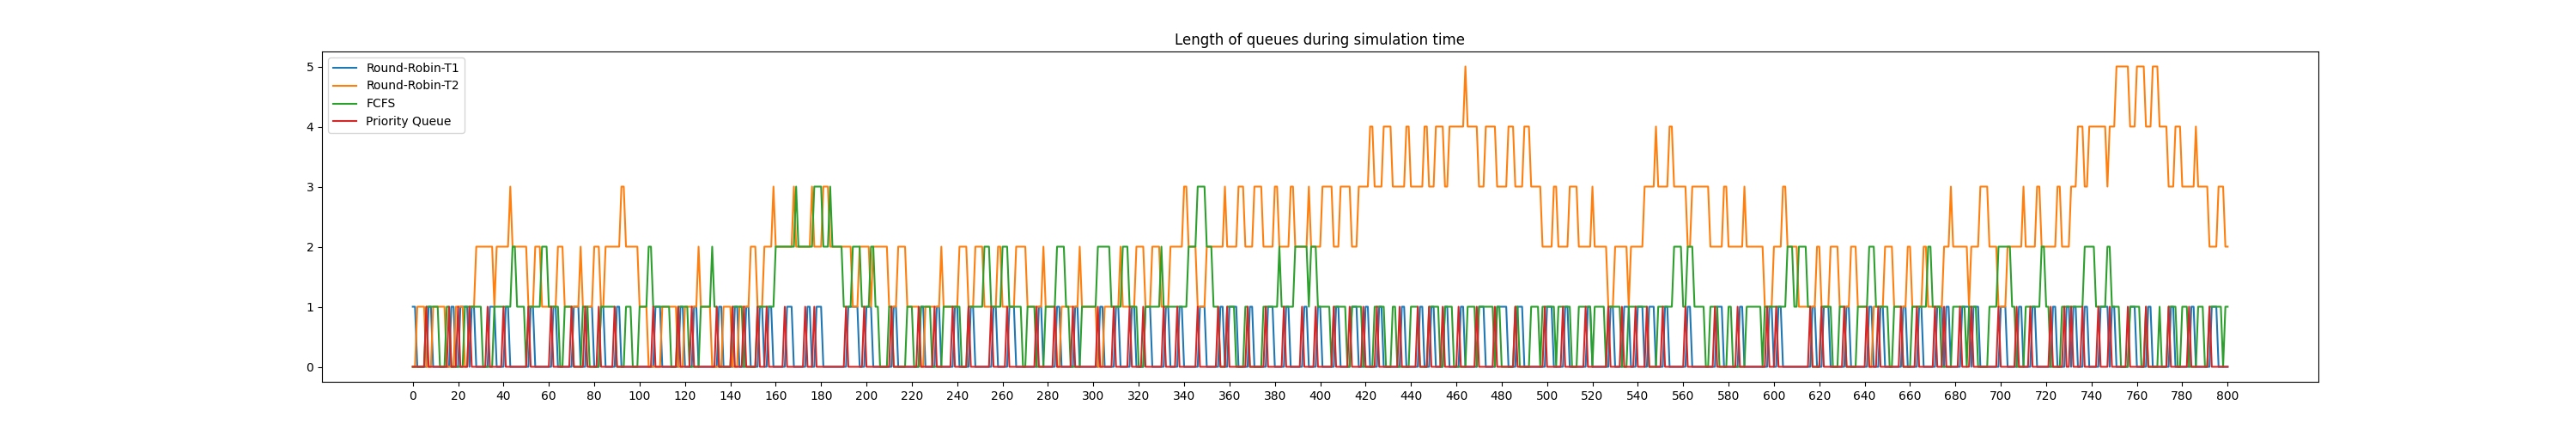
\includegraphics[width=\columnwidth]{figs/loq/queue-len-X-8-Y-8-Z-32-N-100-L-800-K-10-T1-2-T2-4.png}
		\caption{ورودی اول}
	\end{subfigure}
	\begin{subfigure}{.5\columnwidth}
		\centering
		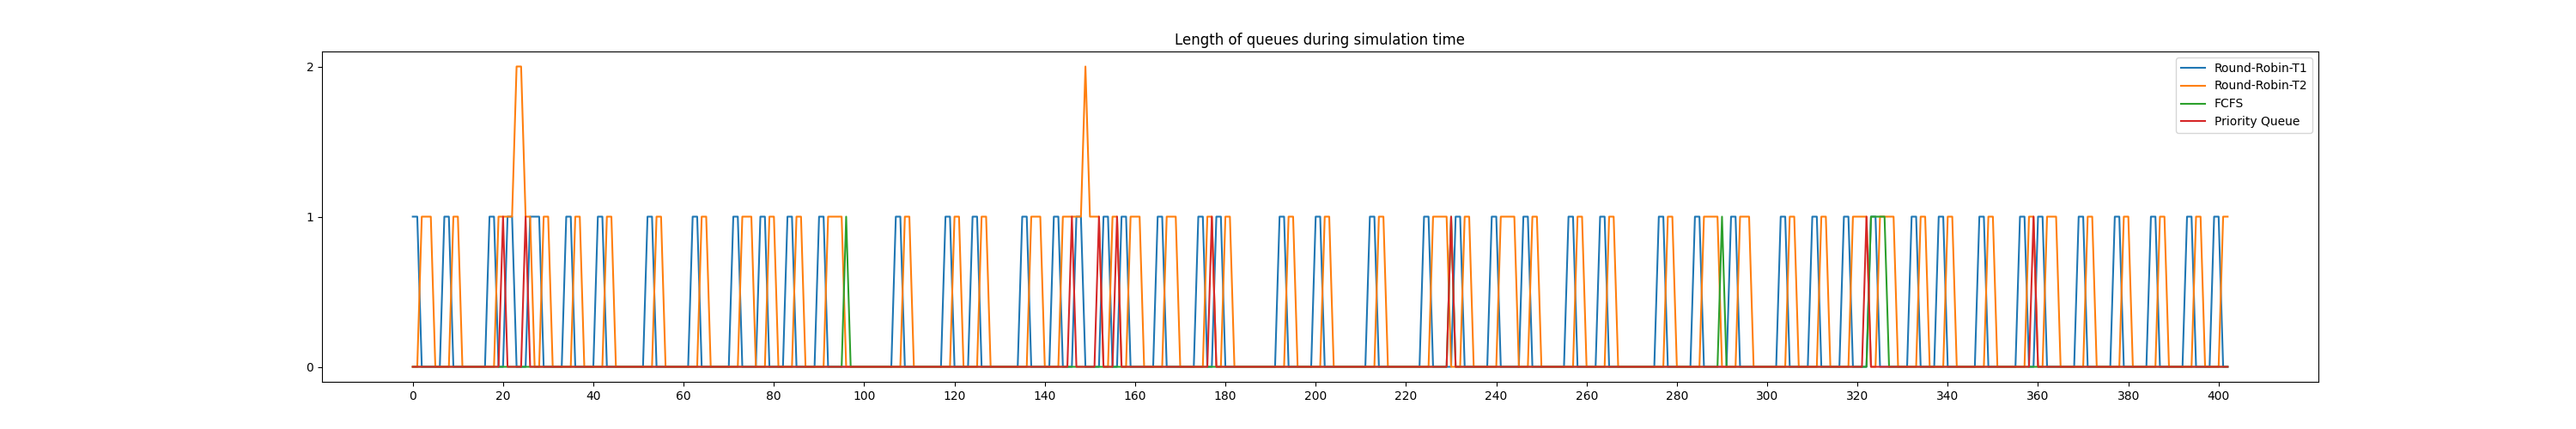
\includegraphics[width=\columnwidth]{figs/loq/queue-len-X-8-Y-4-Z-32-N-50-L-800-K-10-T1-2-T2-4.png}
		\caption{ورودی دوم}
	\end{subfigure}
	\vskip\baselineskip
	\begin{subfigure}{.5\columnwidth}
		\centering
		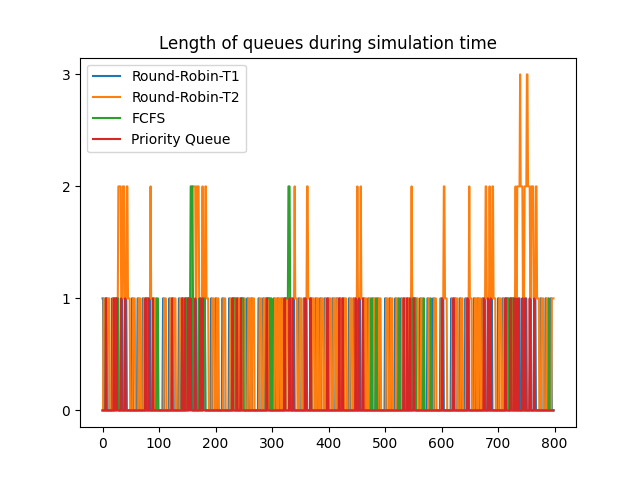
\includegraphics[width=\columnwidth]{figs/loq/queue-len-X-8-Y-6-Z-16-N-100-L-800-K-10-T1-2-T2-4.png}
		\caption{ورودی سوم}
	\end{subfigure}
	\begin{subfigure}{.5\columnwidth}
		\centering
		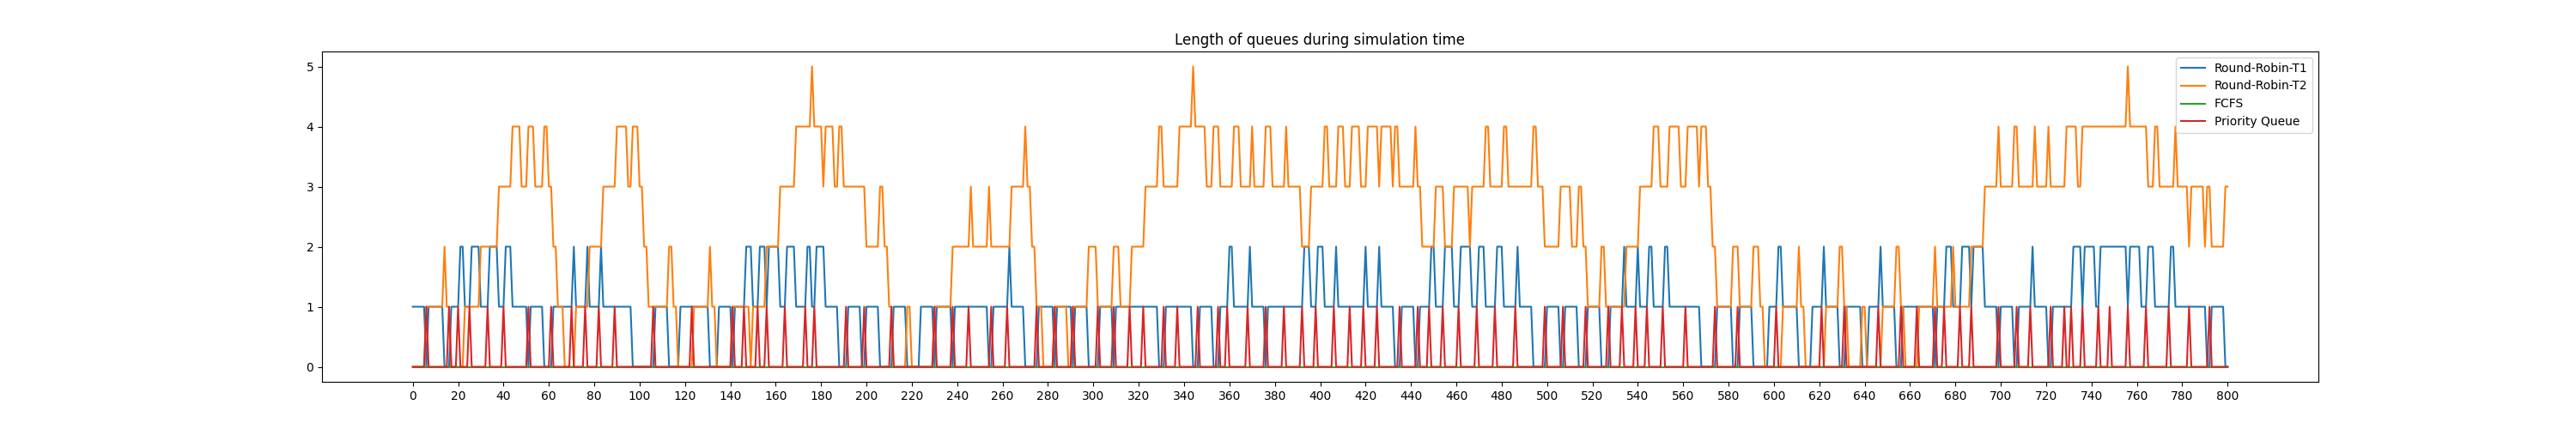
\includegraphics[width=\columnwidth]{figs/loq/queue-len-X-8-Y-8-Z-32-N-100-L-800-K-10-T1-6-T2-8.png}
		\caption{ورودی چهارم}
	\end{subfigure}
	\caption{طول صف‌های لایه اول و دوم به‌ازای ورودی‌های مختلف}
	\label{fig:loq}
\end{figure}

\subsection{میانگین زمان صرف‌شده در صف‌ها}
نمودار زمان صرف‌شده در صف‌ها در شکل \ref{fig:tsq} آمده است.

\begin{figure}[h!]
	\begin{subfigure}{1\columnwidth}
		\centering
		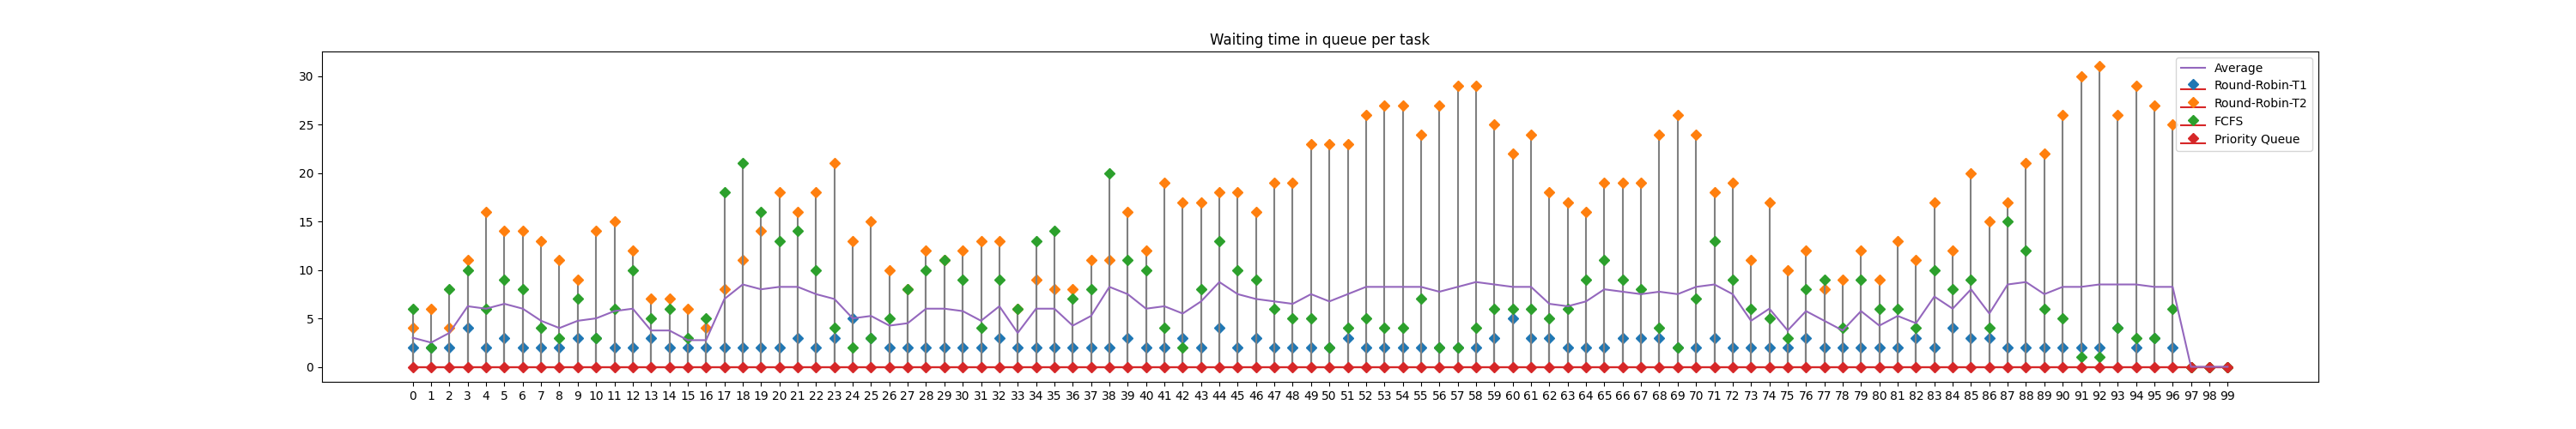
\includegraphics[width=\columnwidth]{figs/tsq/task-in-queue-X-8-Y-8-Z-32-N-100-L-800-K-10-T1-2-T2-4.png}
		\caption{ورودی اول}
	\end{subfigure}
	\vskip\baselineskip
	\begin{subfigure}{1\columnwidth}
		\centering
		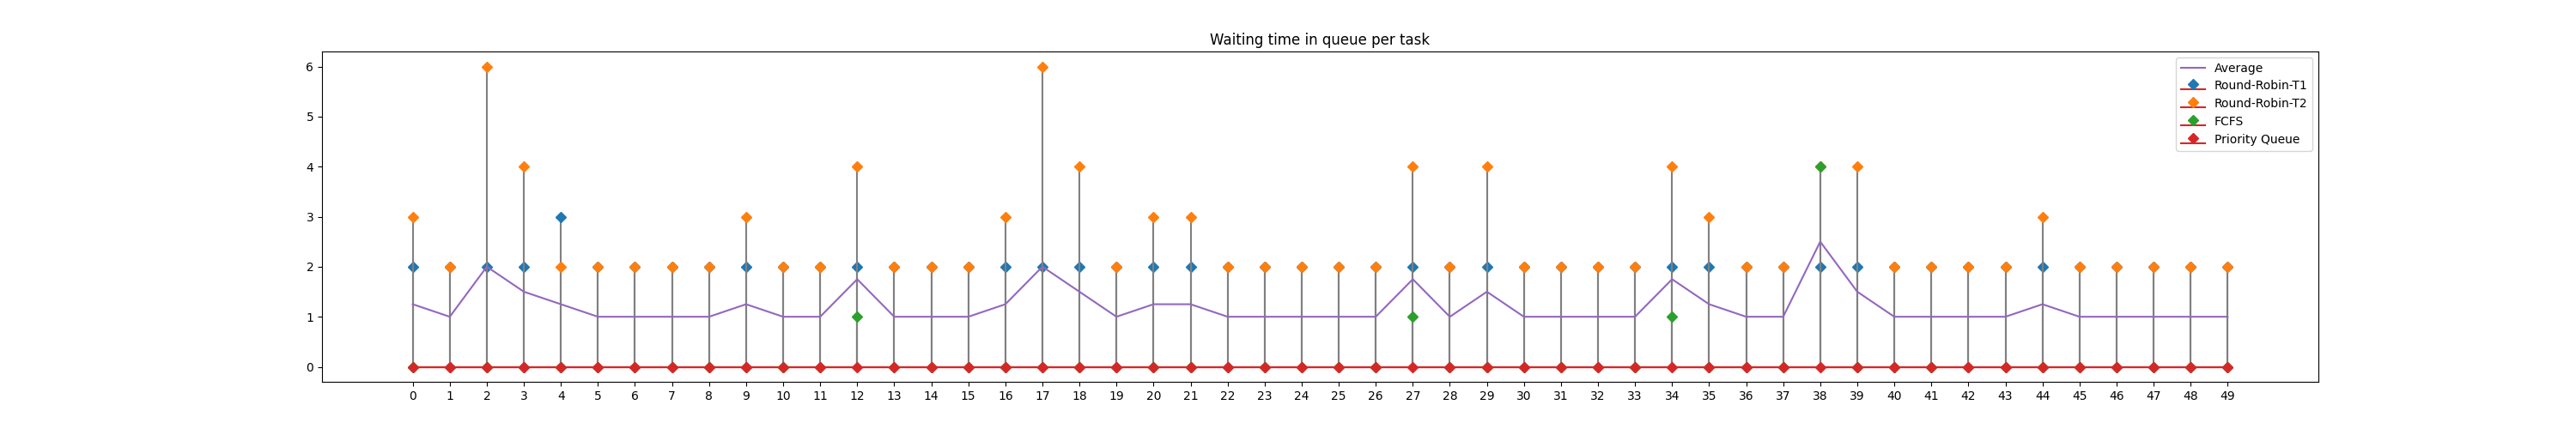
\includegraphics[width=\columnwidth]{figs/tsq/task-in-queue-X-8-Y-4-Z-32-N-50-L-800-K-10-T1-2-T2-4.png}
		\caption{ورودی دوم}
	\end{subfigure}
	\vskip\baselineskip
	\begin{subfigure}{1\columnwidth}
		\centering
		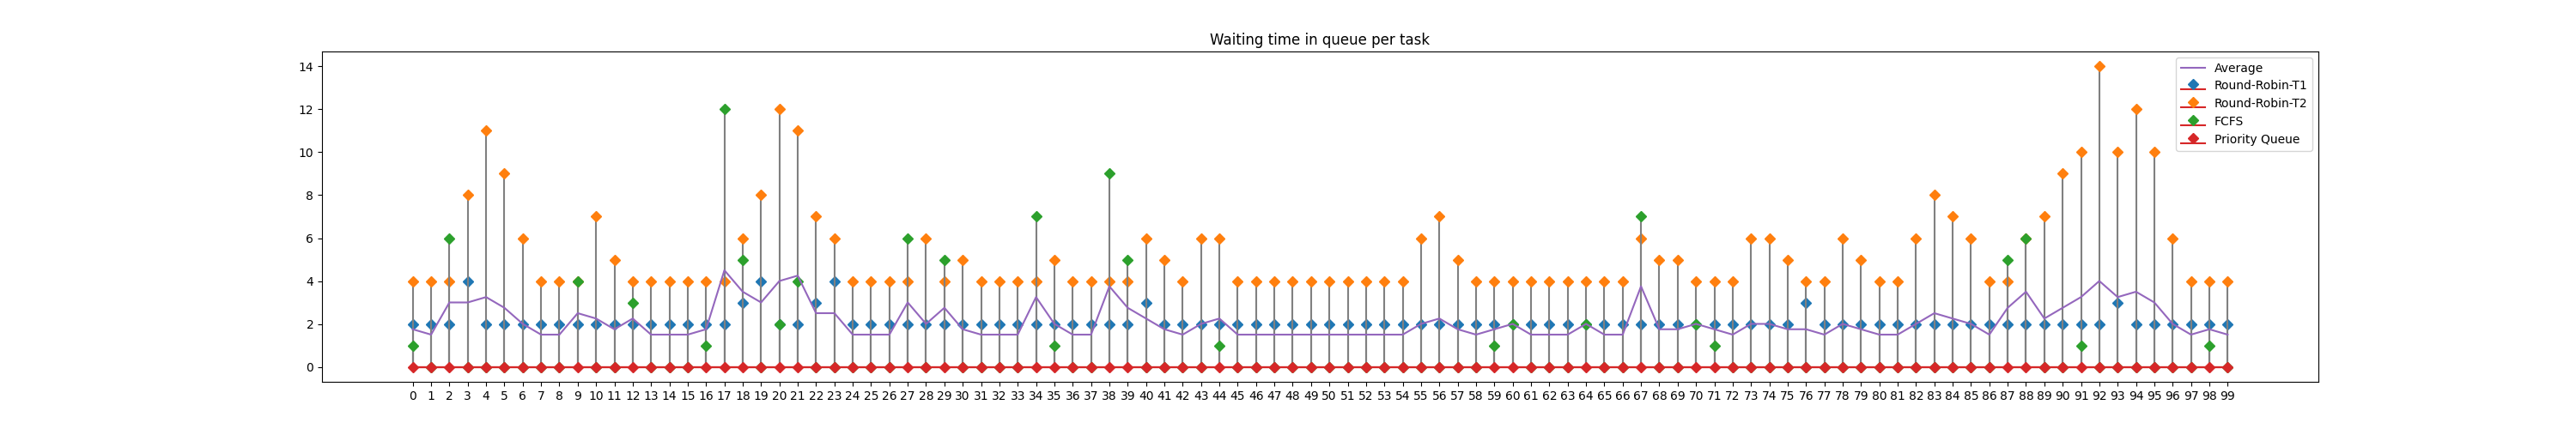
\includegraphics[width=\columnwidth]{figs/tsq/task-in-queue-X-8-Y-6-Z-16-N-100-L-800-K-10-T1-2-T2-4.png}
		\caption{ورودی سوم}
	\end{subfigure}
	\vskip\baselineskip
	\begin{subfigure}{1\columnwidth}
		\centering
		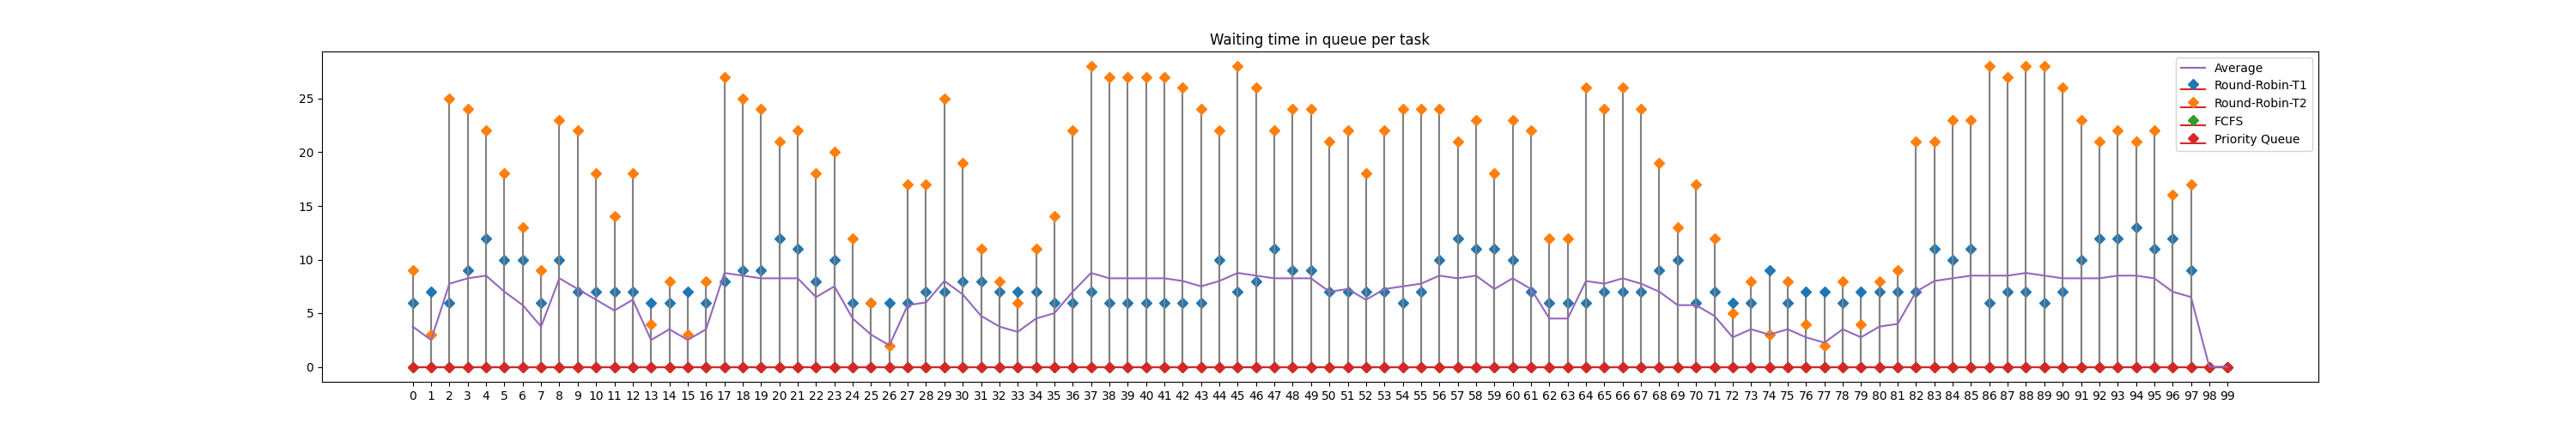
\includegraphics[width=\columnwidth]{figs/tsq/task-in-queue-X-8-Y-8-Z-32-N-100-L-800-K-10-T1-6-T2-8.png}
		\caption{ورودی چهارم}
	\end{subfigure}
	\caption{زمان صرف‌شده در صف‌های مختلف به‌ازای ورودی‌های مختلف}
	\label{fig:tsq}
\end{figure}

\subsection{میزان بهره‌وری پردازنده}
میزان بهره‌وری پردازنده در ورودی اول $100\%$، در ورودی دوم $78.0\%$، در ورودی سوم $80.2\%$ و در ورودی چهارم $98.5\%$ است.

\subsection{بهبود میانگین زمان صرف‌شده در صف‌ها}
تودو

\subsection{درصد پردازه‌های منقضی‌شده}
درصد پردازه‌های منقضی‌شده در ورودی اول $20.0\%$، در ورودی دوم $0.0\%$، در ورودی سوم $1.0\%$ و در ورودی چهارم $28.0\%$ است.

\end{document}
